% ---------------------------------------------------------------------------
% Initial Situation
\begin{frame}
    \frametitle{Initial Situation}
    \centering
    \includegraphics[width=0.8\linewidth]{../assets/collage_sound_pollution.png}
\end{frame}
% ---------------------------------------------------------------------------

% ---------------------------------------------------------------------------
% Project Goals
\begin{frame}
    \frametitle{Project Goals}
    \begin{columns}
        \column{0.5\textwidth}
        \begin{itemize}[<+->]
            \large
            \item Analyze Audio File
            \item Summarize findings in a PDF
            \item Easy to use
        \end{itemize}
        \column{0.5\textwidth}
        \centering
        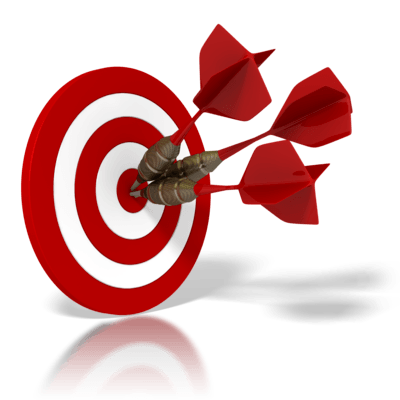
\includegraphics[width=1\linewidth]{../assets/target.png}
    \end{columns}
\end{frame}
% ---------------------------------------------------------------------------
% ---------------------------------------------------------------------------

% Audio Files
\begin{frame}
    \frametitle{Audio Files}
    \centering
    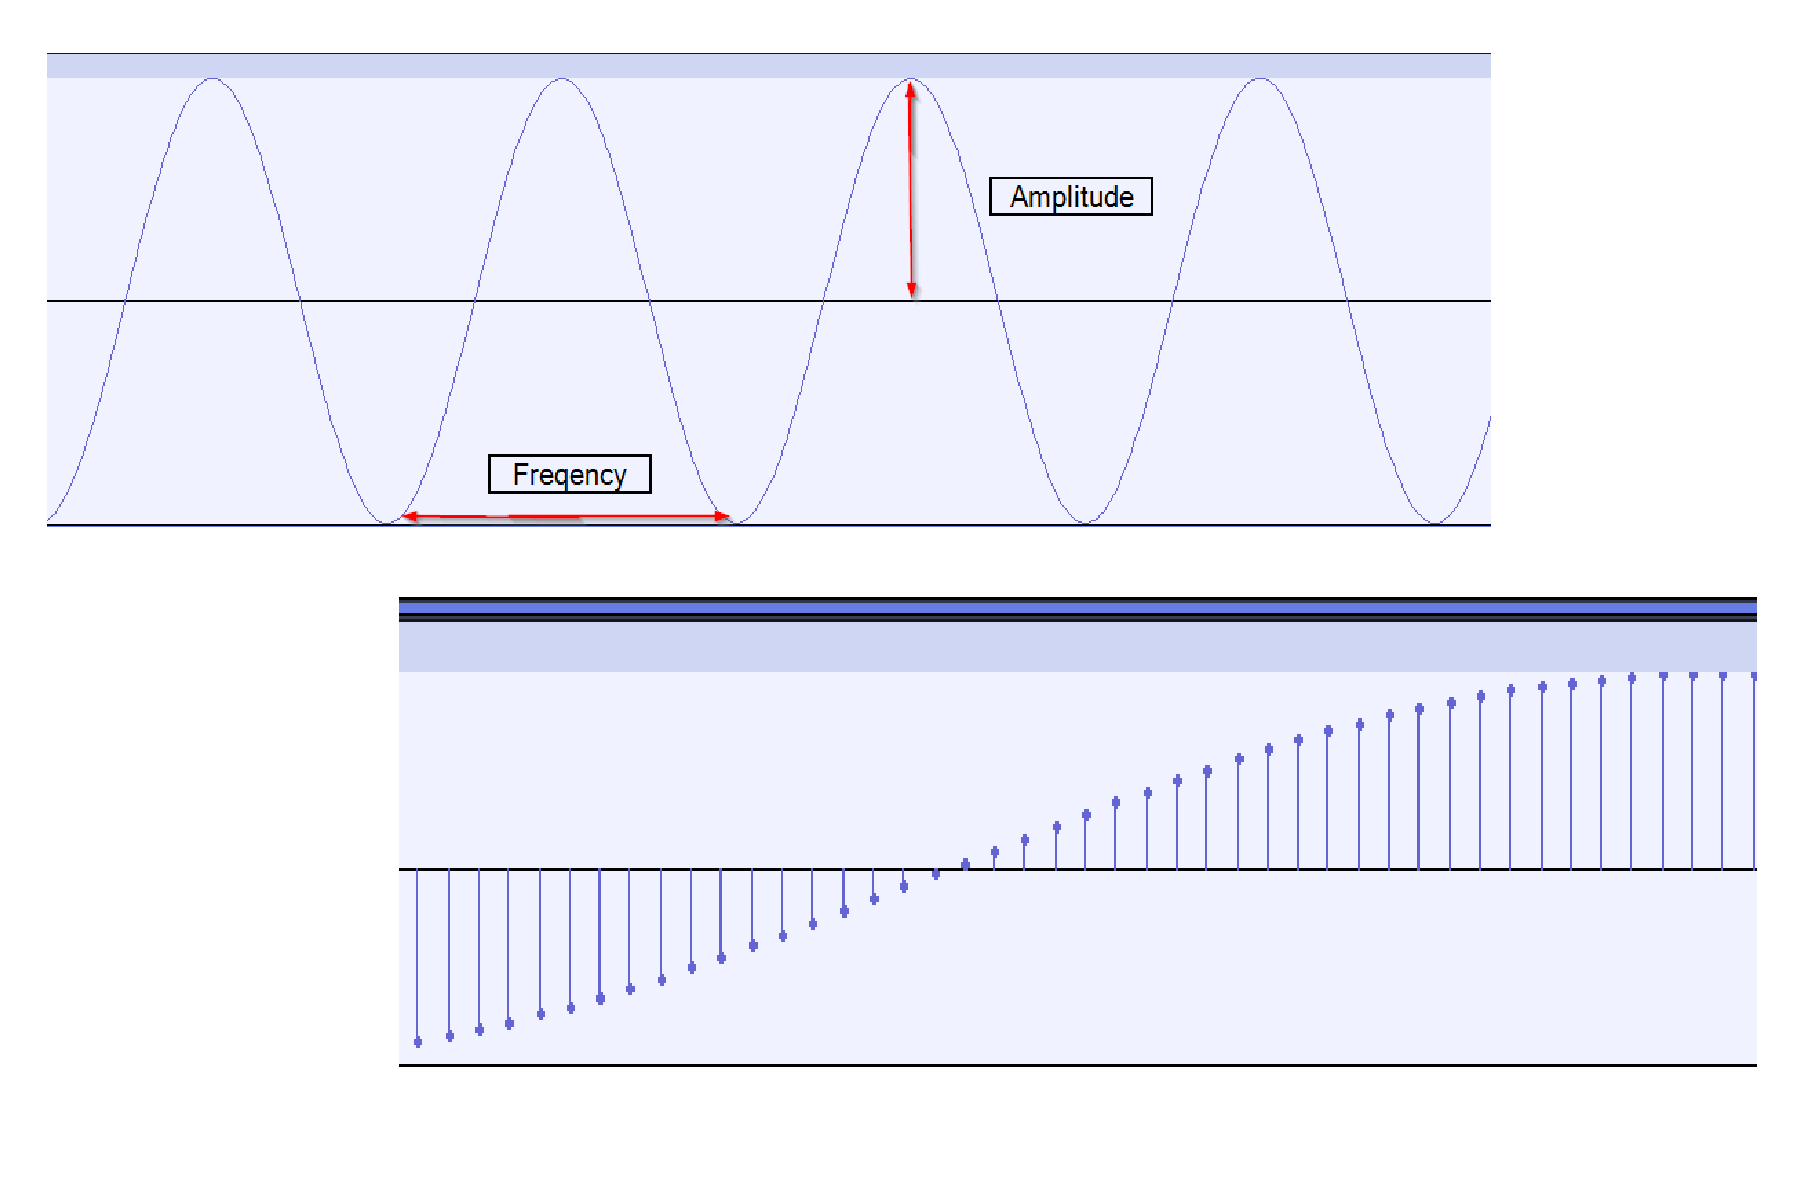
\includegraphics[width=0.8\linewidth]{../assets/audiofile_description.png}
\end{frame}
% ---------------------------------------------------------------------------

% Measuring the Sound Level
\begin{frame}
    \frametitle{Measuring the Sound Level}
    \centering
    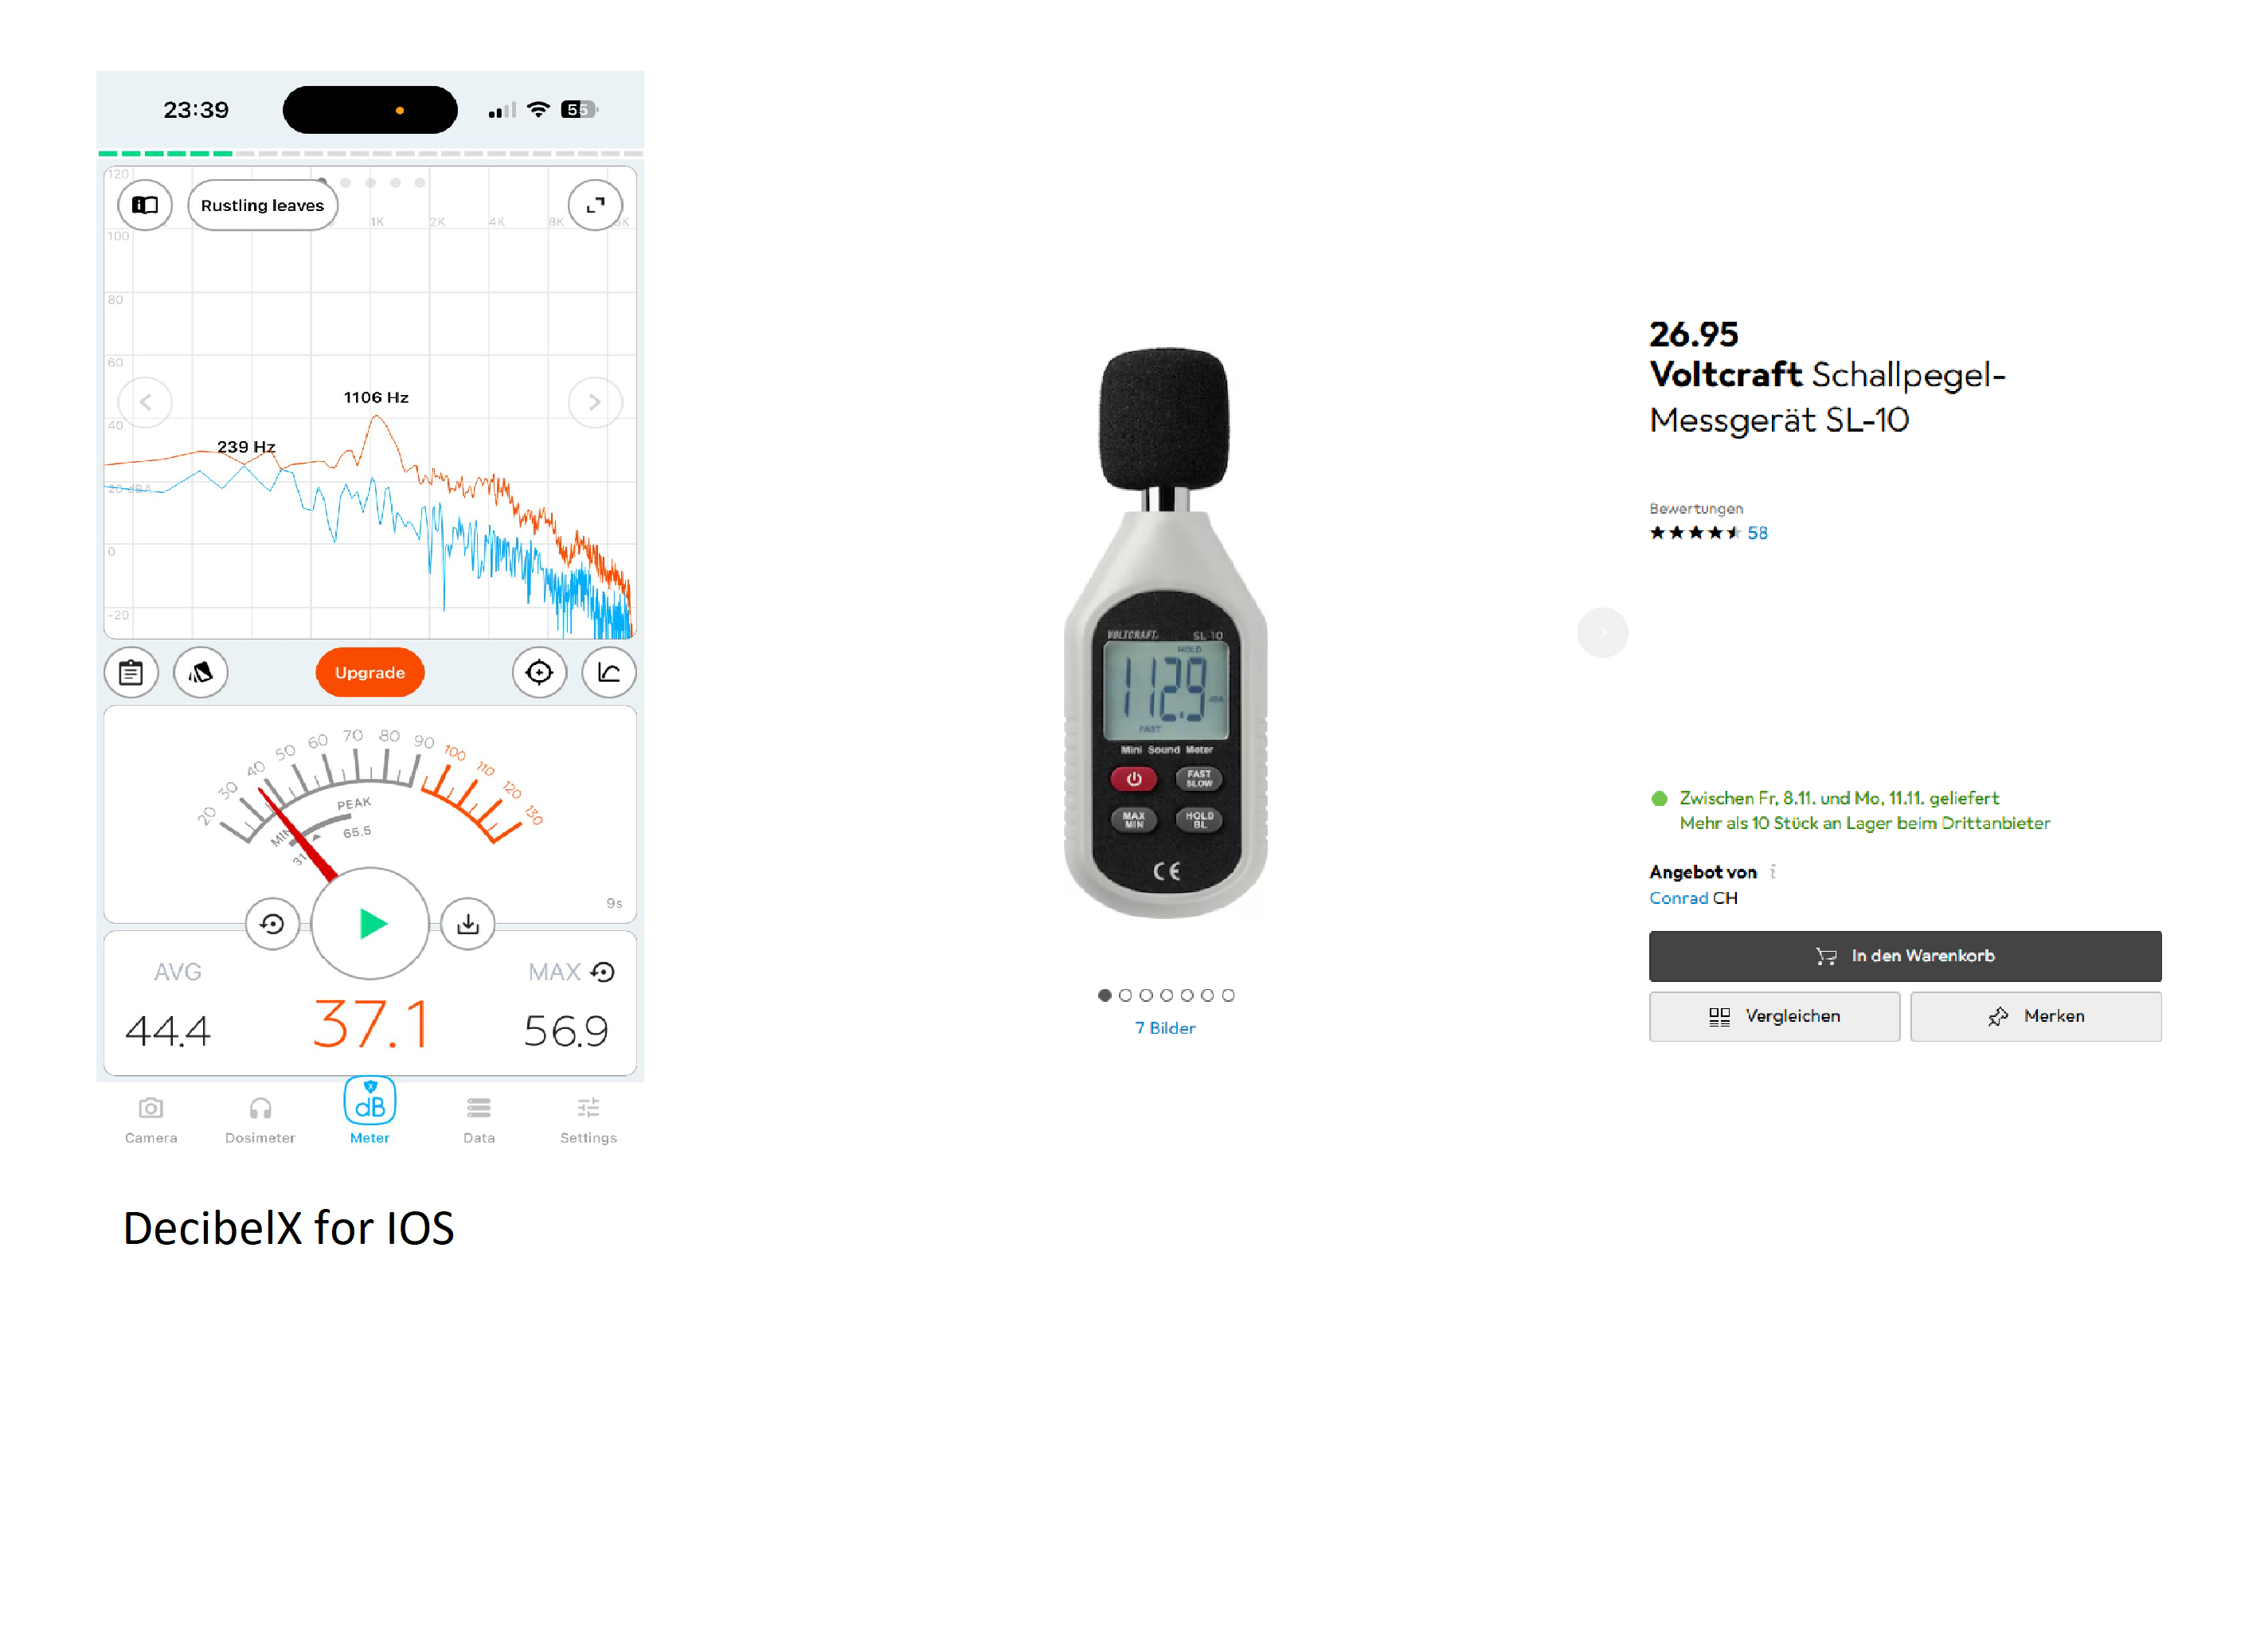
\includegraphics[width=0.6\linewidth]{../assets/measure_sound_level.png}
\end{frame}
% ---------------------------------------------------------------------------

% Requirements
\begin{frame}
    \frametitle{Requirements}
    \begin{itemize}[<+->]
        \large
        \item Take .wav file, threshold and additional reference values as input
        \item Analyze and Summarize 
        \begin{itemize}
            \large
            \item Metadata
            \item Plot
        \end{itemize}
        \item User should not need any Technical know-How
        \item Platform independent
        \item (Multiple Languages)
    \end{itemize}
\end{frame}
% ---------------------------------------------------------------------------

% ---------------------------------------------------------------------------
% Technologies evaluation
\begin{frame}
    \frametitle{Technology evaluation}
    \par\vspace{0.5cm}
    \centering
    \begin{table}[H]
        \centering
        \begin{tabular}{|l|c|c|}
            \hline
            \textbf{Technology} & \textbf{Total score} \\
            \hline
            Kotlin minimal & 74 \\
            \hline
            Kotlin bundled & 56 \\
            \hline
            Web SwiftLaTeX & 82 \\
            \hline
        \end{tabular}
        \label{table:technology_evaluation}
    \end{table}
\end{frame}
% ---------------------------------------------------------------------------